% Preamble
\documentclass[12pt]{article}

\usepackage[utf8]{inputenc}
\usepackage[margin=1in]{geometry} %1in = 2.54cm margin
\usepackage[titletoc,title]{appendix}
\usepackage{amsmath,amsfonts,amssymb,mathtools}
\usepackage[ruled,vlined]{algorithm2e}
\usepackage{import}
\usepackage{xifthen}
\usepackage{pdfpages}
\usepackage{transparent}
\usepackage{calc}
\newcommand{\incfig}[1]{%
\def\svgwidth{\columnwidth}\import{Figures/}{#1.pdf_tex}}
\usepackage{algorithmicx}
\usepackage{algpseudocode}
\usepackage{makecell}
\usepackage{indentfirst}
\usepackage{caption}
\usepackage{subcaption}
\usepackage{mathptmx}
\usepackage[symbol]{footmisc}
\usepackage{wrapfig}
\usepackage{dirtytalk}
\usepackage[backref=true]{biblatex}
\usepackage{hyperref}
\DefineBibliographyStrings{english}{backrefpage={Cited on p.}, backrefpages={Cited on pp.}}
\usepackage{tablefootnote}
\usepackage{fancyhdr}
\usepackage[export]{adjustbox}
\usepackage{sectsty}
\sectionfont{\large}
\subsectionfont{\normalsize}
\subsubsectionfont{\footnotesize}
\pagestyle{fancy}
\renewcommand{\headrulewidth}{0pt}

\lhead{\footnotesize{Computational Aeroacoustics Absorbing Boundary Conditions}}
\rhead{\footnotesize{Peter M. Cassidy}}

\renewcommand{\thefootnote}{\fnsymbol{footnote}}
\renewcommand{\figurename}{Fig.}
\usepackage[font=footnotesize,labelfont=bf]{caption}
\captionsetup{labelsep=space}

\addbibresource{references.bib}
\renewcommand*{\bibfont}{\scriptsize}

\linespread{1}




%%%%%%%%%%%%%%%%%%%%%%%%%%%%%%%%%%%%%%%%%%%%%%%%%%%%%%%%%%%%%%%%%



\begin{document}


\begin{figure}
    
\includegraphics[width=0.4\textwidth,right]{Figures/Misc/LULogo.png}
\end{figure}


\begin{titlepage}

   \begin{center}

    	\Large{\textbf{Investigating Absorbing Boundary Conditions for Computational Aeroacoustics Problems}}

       \vspace{0.8cm}

       \footnotesize{Peter M. Cassidy\footnote[1]{Aeronautical Engineering MEng; B725700; Project supervisor: Dr Hao Xia}}


       \textit{Department of Aeronautical and Automotive Engineering,\\
       Loughborough University, Leicestershire LE11 3TU, UK}
       
       \vspace{0.8cm}
     
       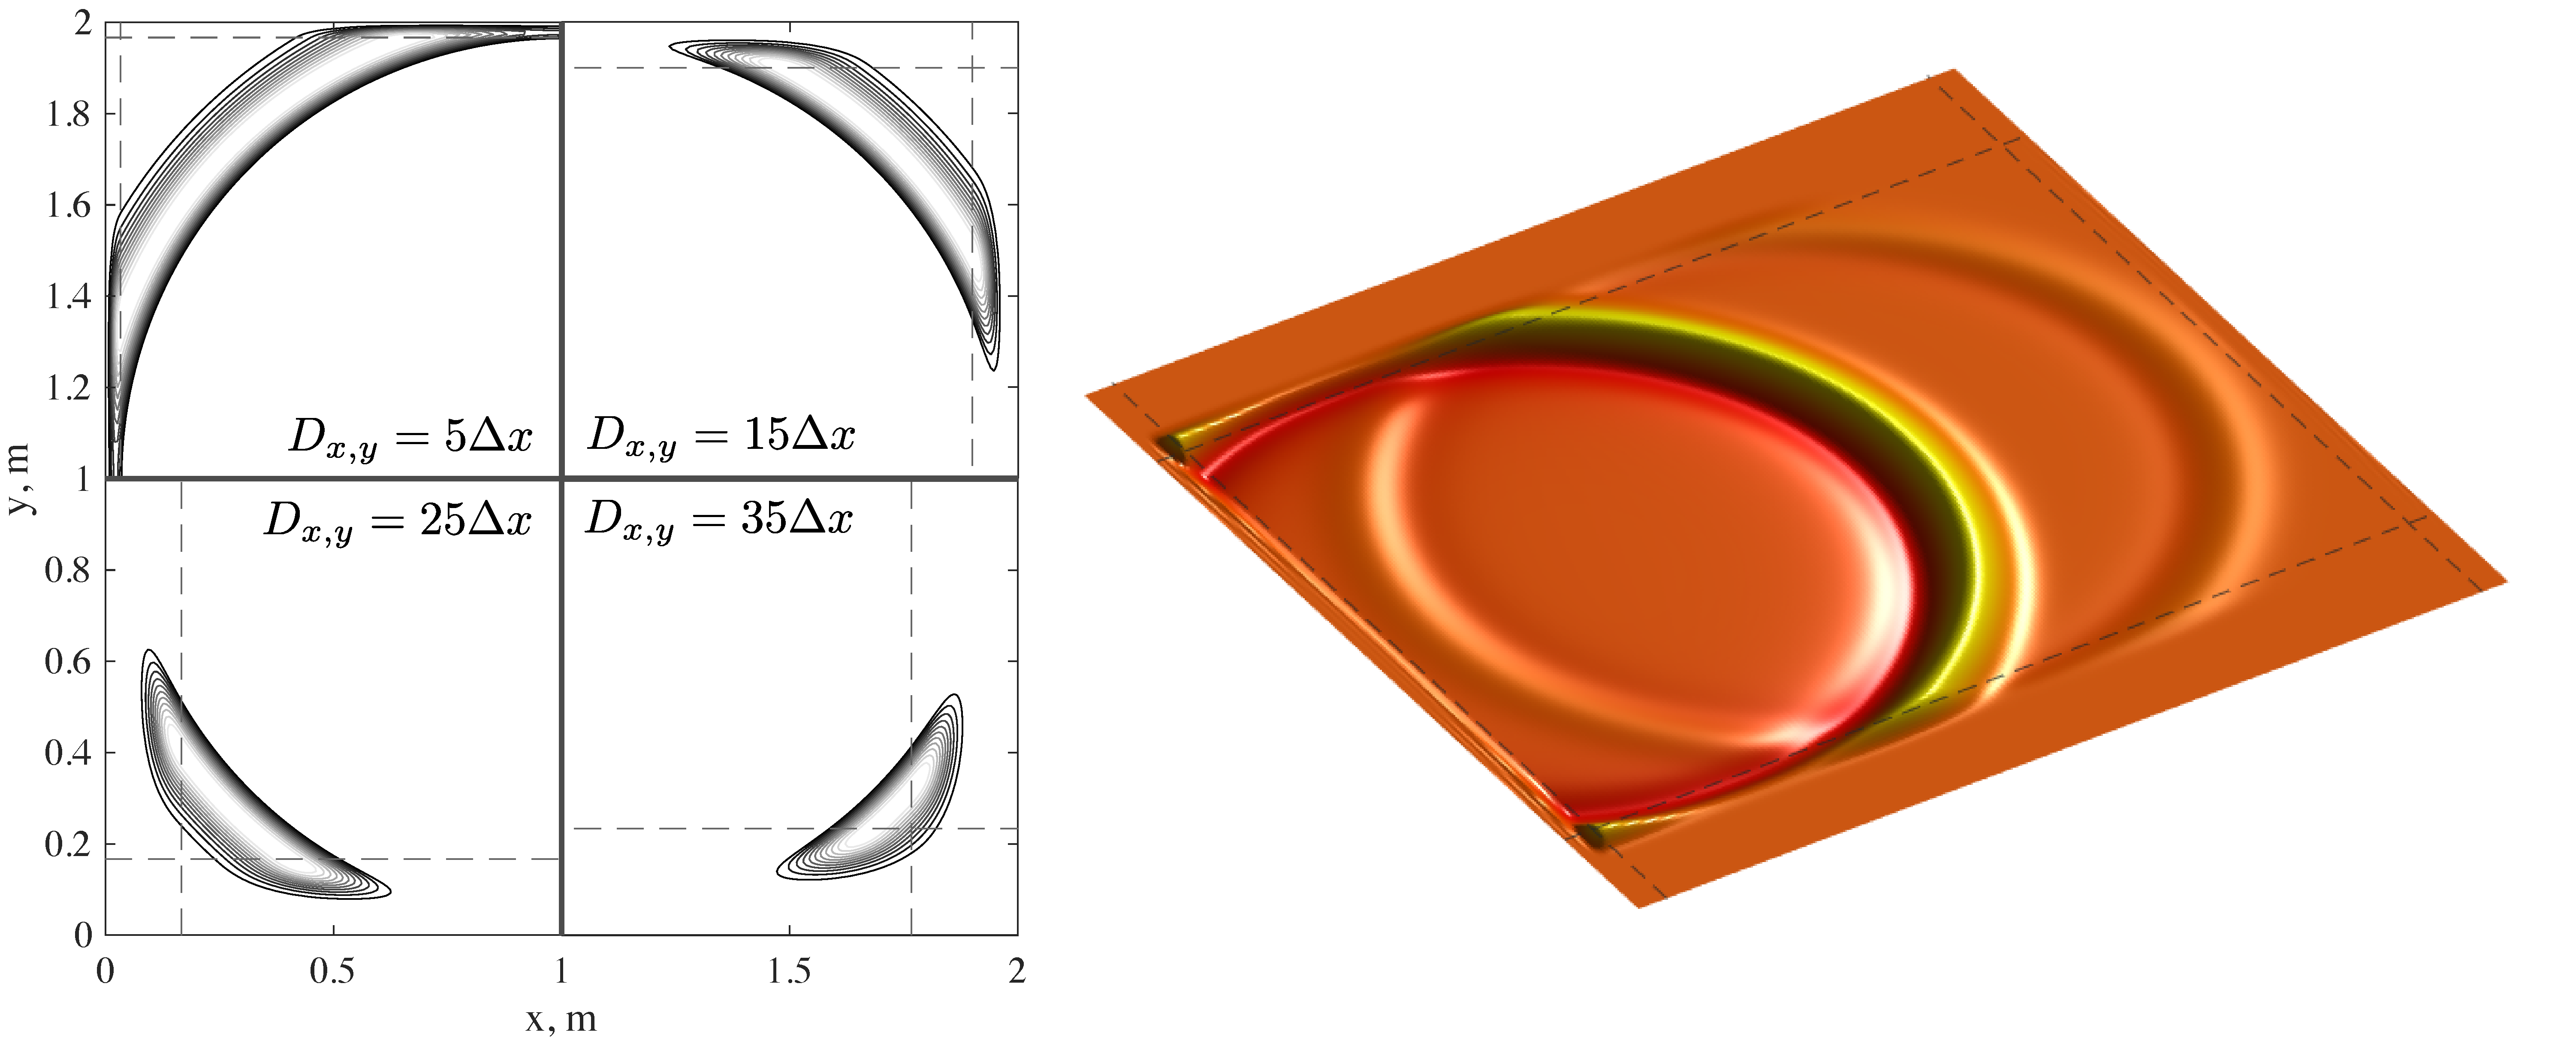
\includegraphics[width=16cm]{Figures/Misc/Summary.eps}
            
            
   \end{center}
   
   Presented in this report are the methods and results of implementing \& optimising a perfectly matched layer boundary condition in a MATLAB-based linearised Euler equation solver. \par
The design of modern turbofan acoustic liners requires accurate prediction of the wave propagation - characterised by the underlying numerical methods. This umbrella term encompasses many individual elements, but the boundary conditions are the focus of the project.
A literature review has concluded that absorbing zone non-reflecting boundary conditions are top performers in their class, and have quite rightly been the subject of reams of research looking to increase prediction accuracy.


When discretised using dispersion relation preserving finite difference schemes and multi-level Adams Bashforth time integration schemes, the developed solver accurately predicts wave propagation in the domain, and the absorption of outgoing waves in the perfectly matched layer zone. The solver has shown to perform well when subject to NASA-sponsored CAA workshop problems, and predicts similarly to more mature research solvers.


The results indicate that there exists a finite set of BC parameter combinations that produce minimal domain error, and these conditions align relatively well with those that have been analytically derived in other research. Further work is necessary to assess these combinations on another research solver in order to solidify the conclusions.


\end{titlepage}
\newpage

\section{Introduction} \label{IntroductionSection}

\subsection{Motivation and Relevance}

Noise emissions from air traffic in areas close to airports is a constant battle. The new aero-engines in development at Rolls-Royce, General Electric, and Pratt \& Whitney have increasingly larger bypass ratios to increase overall efficiency. This ultimately leads to larger fans and a growth in nacelle diameter. Previously, engine manufacturers have simply increased the inlet and bypass lengths proportionally with the nacelle diameter, but the associated drag and weight penalties of doing this for next generation engines is unfeasible. Therefore, there is physically less nacelle space for acoustic liners, requiring more efficient liner damping to meet emissions regulations. Compounding this is the fact that larger engines produce lower blade passing frequencies (BPF) which require deeper liners to attenuate the noise, and thus thicker nacelles. This is again not possible due to drag and weight penalties. So new, highly-complex liner concepts are required. An example of such a liner is the Special Acoustic Absorber (SAA), developed by \textcite{redmann2013aeroacousticliner} in 2013. The added complexity of these new liners enforces the need for CAA solvers with clever features, such as efficient non-reflecting boundary conditions (NRBCs). These features are parameterised to the effect that specific combinations of parameters impact the accuracy of the resolved wave propagation inside the domain. 



\subsection{General Aim and Scope}
The primary aim of this project is to investigate a specific non-reflecting boundary condition (NRBC) formulation for use in truncating a computational aeroacoustics domain. The aim is constituted of a number of objectives, including:

\begin{enumerate}
\itemsep0em
\item Accurately \textbf{discretise} complex \textbf{PDEs} using CAA-relevant schemes - governing Euler equations require discretising in space and time using aeroacoustic-optimised formulations
\item Write a \textbf{linearised solver} in MATLAB to predict wave propagation problems - commercial solvers do not yet offer enough flexibility for integrating innovative BCs
\item Implement absorbing zone \textbf{NRBCs}
\item \textbf{Benchmark} the solver against \textbf{workshop problems} - NASA-published aeroacoustics workshops for solver validation
\item Determine \textbf{optimal parameters} for the NRBC implementation - considering induced-error from combinations of parameters
\end{enumerate}

The listed objectives ensure a rigorous and thorough approach that delivers tangible results. 

\newpage

\subsection{Design Context}


The 'optimised' boundary condition parameters sought after in this report could be used in a more matured research solver for exploring unique and innovative acoustic liners. The potential cash impact, then, is two-fold. Firstly computational expenses are reduced by using efficient BC parameters - as less grid points are solved. Secondly, costs can be cut by decreasing drag and weight, which is enabled by shorter/thinner nacelles, which is enabled by space-efficient liners, which is enabled by accurate cutting-edge CAA methods. The end result is beneficial in both a holistic and cash sense.


\subsection{Report Structure and Conventions}

The report structure is illustrated in Figure \ref{fig:ReportStructure}, and follows a rough layout of background \& literature review, methodology, results, and conclusion. 

\begin{figure}[h!]
\centering
\makebox[0pt]{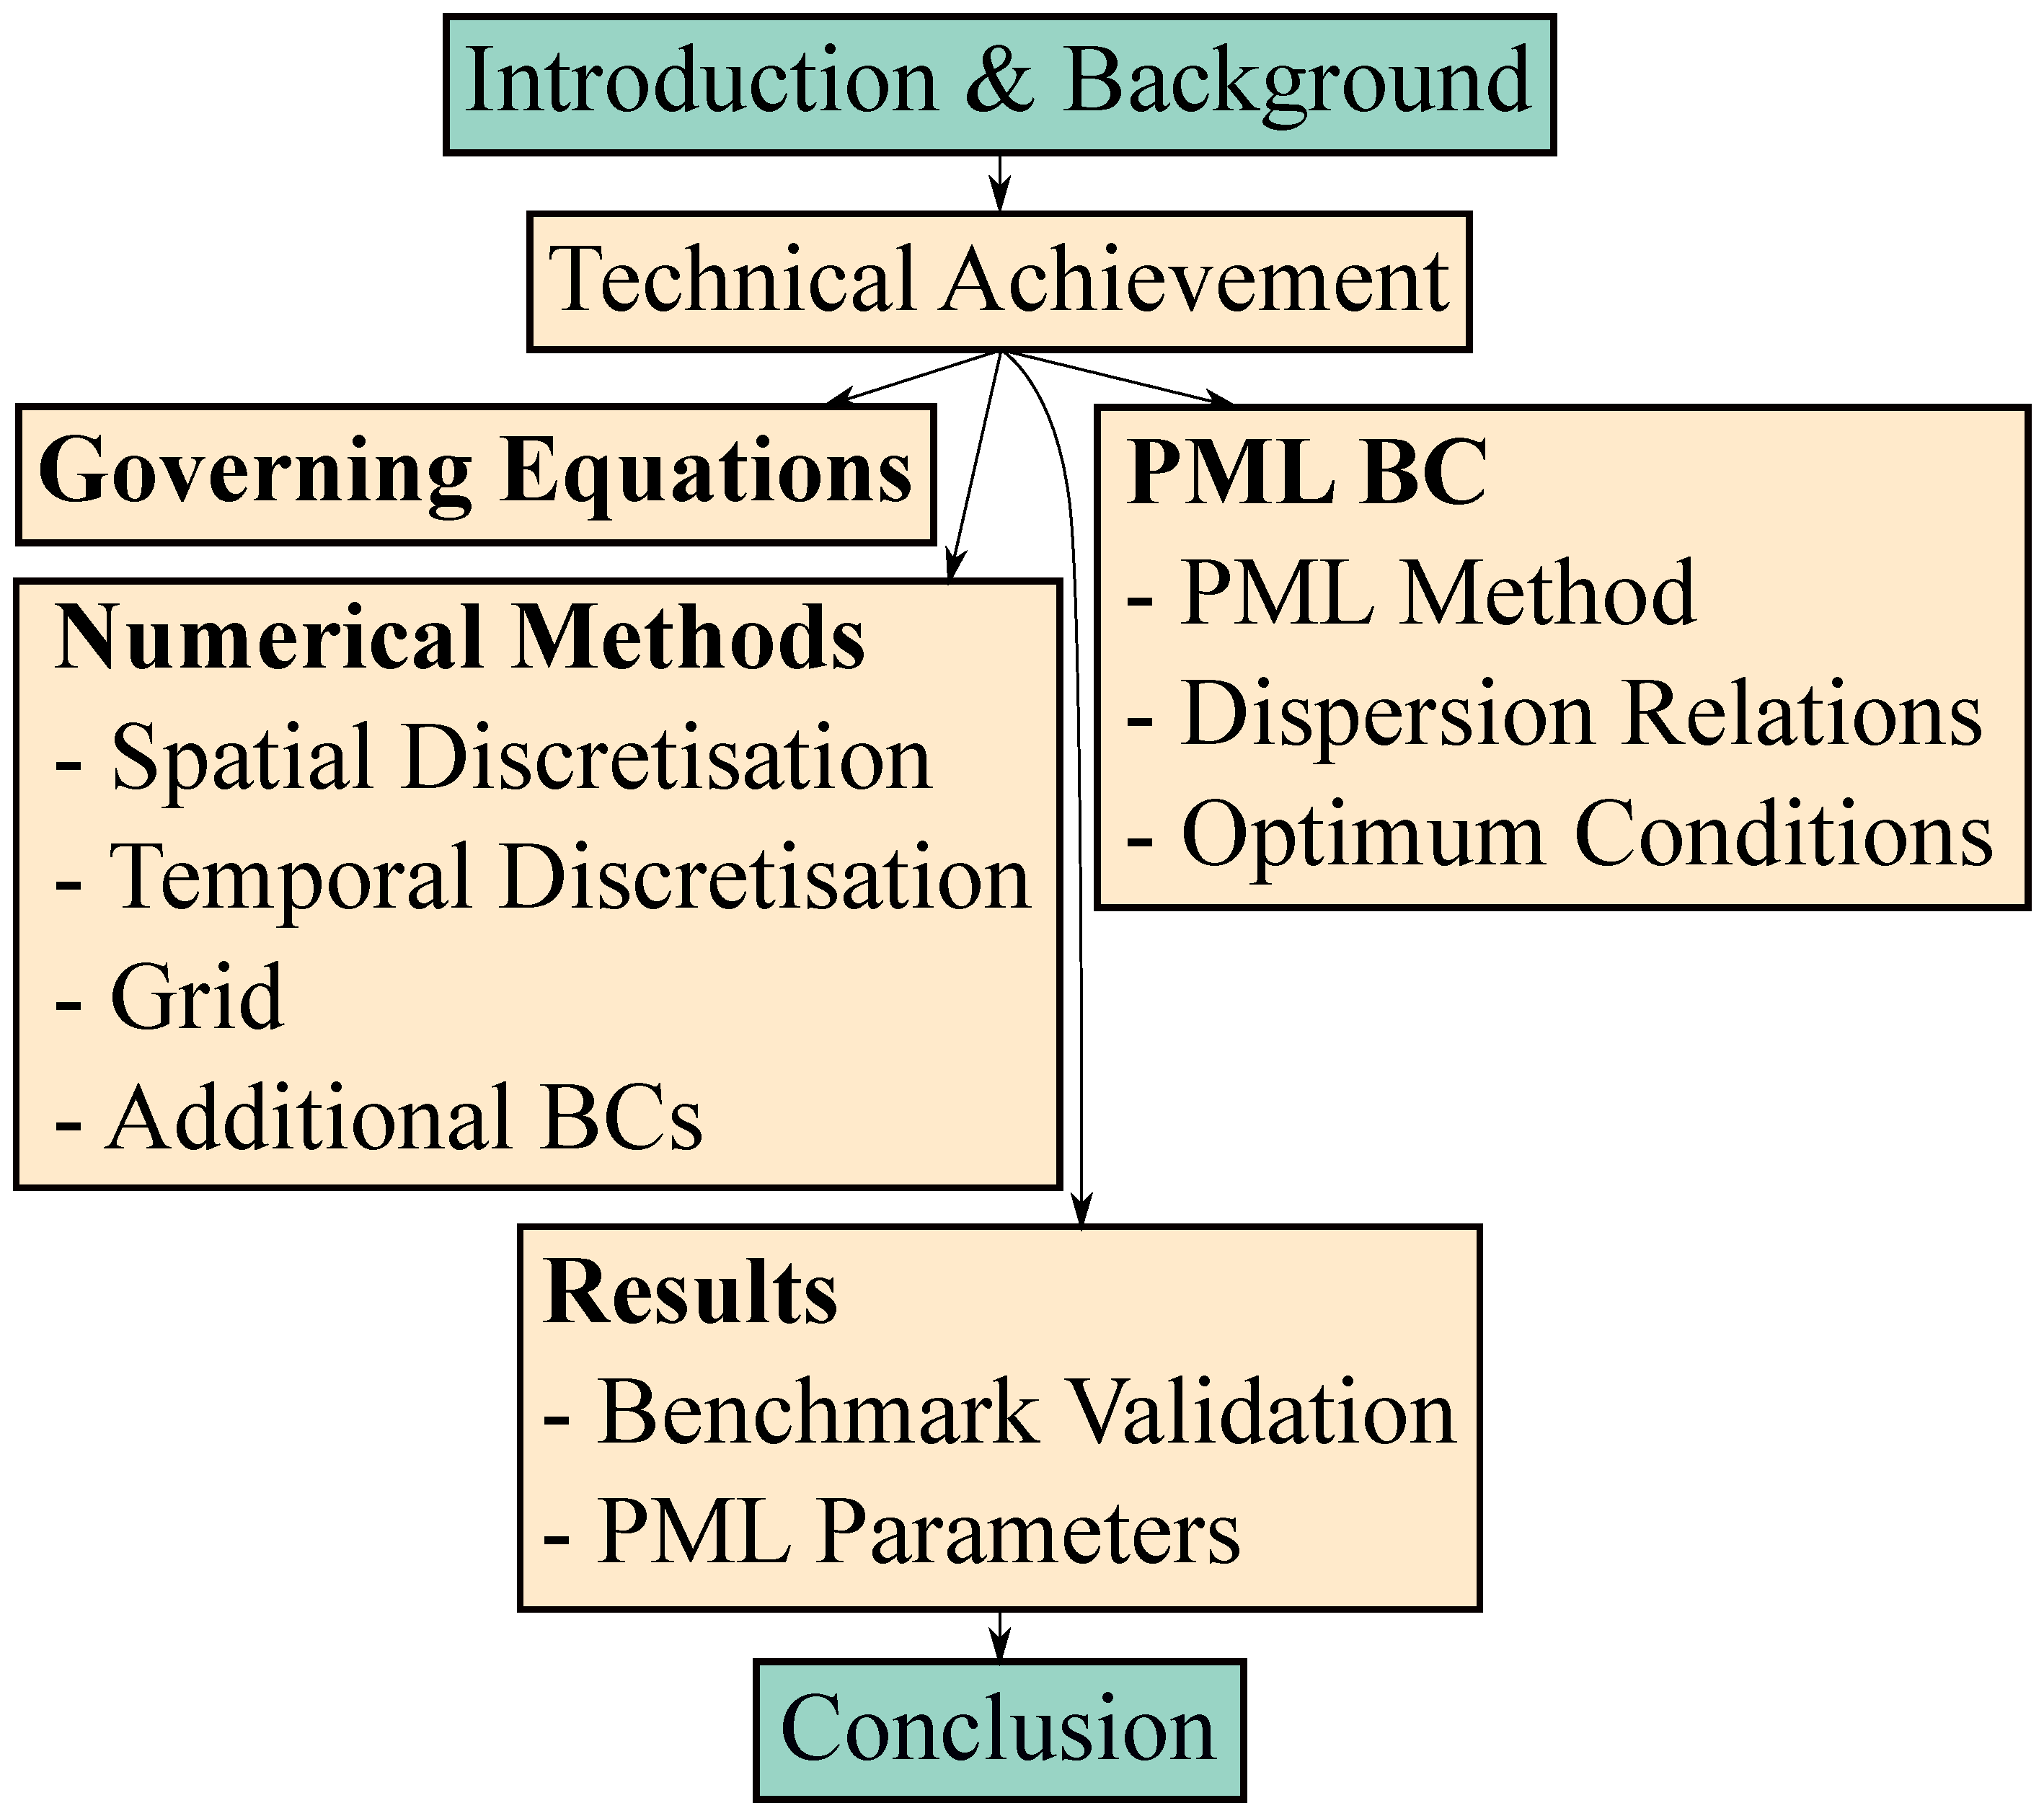
\includegraphics[width=8cm]{Figures/IntroBackground/ReportStructure.eps}}
\caption{Report Structure.}
\label{fig:ReportStructure}
\end{figure}

For methodology, first the governing Euler equations are massaged into a usable form, and then augmented with the perfectly matched layer (PML) boundary condition. The dispersion relations of two PML formulations are assessed for stability, and analytically derived optimum conditions from a source are addressed. The numerical methods for computational implementation are then compared and described, with spatial \& temporal discretisation, grid setup, and additional boundary conditions. The written solver is then validated against a set of NASA benchmark initial conditions, and then the effects of the BC parameters are investigated. The results are summarised and conclusions are drawn to deliver recommendations and further work.

4 field variables are referred to in this report: density $\rho$, velocity in the $x-$direction $u$, velocity in the $y-$direction $v$, and pressure $p$. The freestream Mach number is also defined as $M$. All other symbols are either defined as they appear, or take on their standard definition within engineering and aeroacoustics.

All figures created in this report have been the sole work of the student.
\clearpage

\section{Background} \label{BackgroundSection}

\say{To ensure good quality global CAA solutions, the outer boundaries of the computational domain must be transparent to all outgoing waves} - \textcite{tam193DRP}


Generally speaking, within computational aeroacoustics there are a number of categories for solving sound problems. Firstly there are the acoustic analogies / integral approaches (Lighthill's analogy \cite{lighthill1952onsoundsgenerated}, Ffowcs Williams-Hawkings analogy \cite{ffowcswilliams1969soundgenerationturb}, Curle analogy \cite{curle1955influencesolid}, Kirchhoff-Helmholtz integral \cite{godin1996kirchhoffhelmholtz}), where the propagation of acoustics into the far field is calculated from knowing the flow field variables near the source. Secondly there is the hybrid approach (\textcite{hardin1994acousticsplitting}, \textcite{shen1999commentpopeformulation}, \textcite{ekaterinaris1999newformulationhardinpope}) where the computational domain is decoupled into a flow field and acoustic field so that differing equations and numerical methods can be used to solve for each sub-domain (which vary substantially in scale). The flow field is achieved through a standard CFD solver using either steady-state (RANS) or transient (LES, DES, URANS) solutions. The noise source terms are extracted from the mean flow field\footnote[1]{this is a vast oversimplification, however, a noise source investigation is beyond the scope of this project} and then fed to an acoustic propagation solver. Thirdly there is the linear and nonlinear wave propagation approach using finite difference schemes, which covers a large area of the CAA research space (\textcite{tam2012computational}, \textcite{zingg1996reviewFD}, \textcite{kubratskii2004reviewcaaalgo}). With this approach, partial differential equations (PDEs) describing wave propagation are discretised in space and time to resolve large bandwidths of wavenumbers\footnote[2]{wavenumber being the spatial equivalent of a wave's frequency} with minimal error. Lastly, there is a batch of alternative methods including: lattice gas automata (LGA) \cite{doolen1991LGM}, finite element methods (FEM) \cite{peyret2001FEMCAA}, and boundary element methods (BEM) \cite{kirkup2019BEMCAA} - which are less common within CAA. The third approach of finite difference schemes for linearised governing equations is to be used for this project - as this offers the greatest flexibility in terms of investigating novel boundary conditions.


Acoustic problems as presented in the context of this project are typically within unbounded domains in real-life. Simulating these problems computationally requires the domain to be bounded or truncated. Within typical open-domain CFD problems, the subject of boundary conditions is trivial - the farfield is set far enough away from the body/geometry to remove interference and any propagating flow phenomena are simply dissipated throughout the domain farfield. When considering aeroacoustics, low-dispersion, low-dissipation methods are required which allow for waves to propagate for very large distances within the domain. Therefore, it is important for boundary conditions to be integrated which allow for the waves to outflow through the domain boundaries without affecting the inner domain, to be able to constrain the problem to a sensible size. Otherwise, the computational effort required for a solution with a far enough boundary to avoid reflections is nonsensical. The solution is to implement non-reflecting boundary conditions (NRBC), as illustrated by Figures \ref{fig:UnboundedDomain} and \ref{fig:TruncatedDomain}.


\begin{figure}[h]
    \centering
    \begin{subfigure}[h]{0.47\textwidth}
        \centering
        \makebox[0pt]{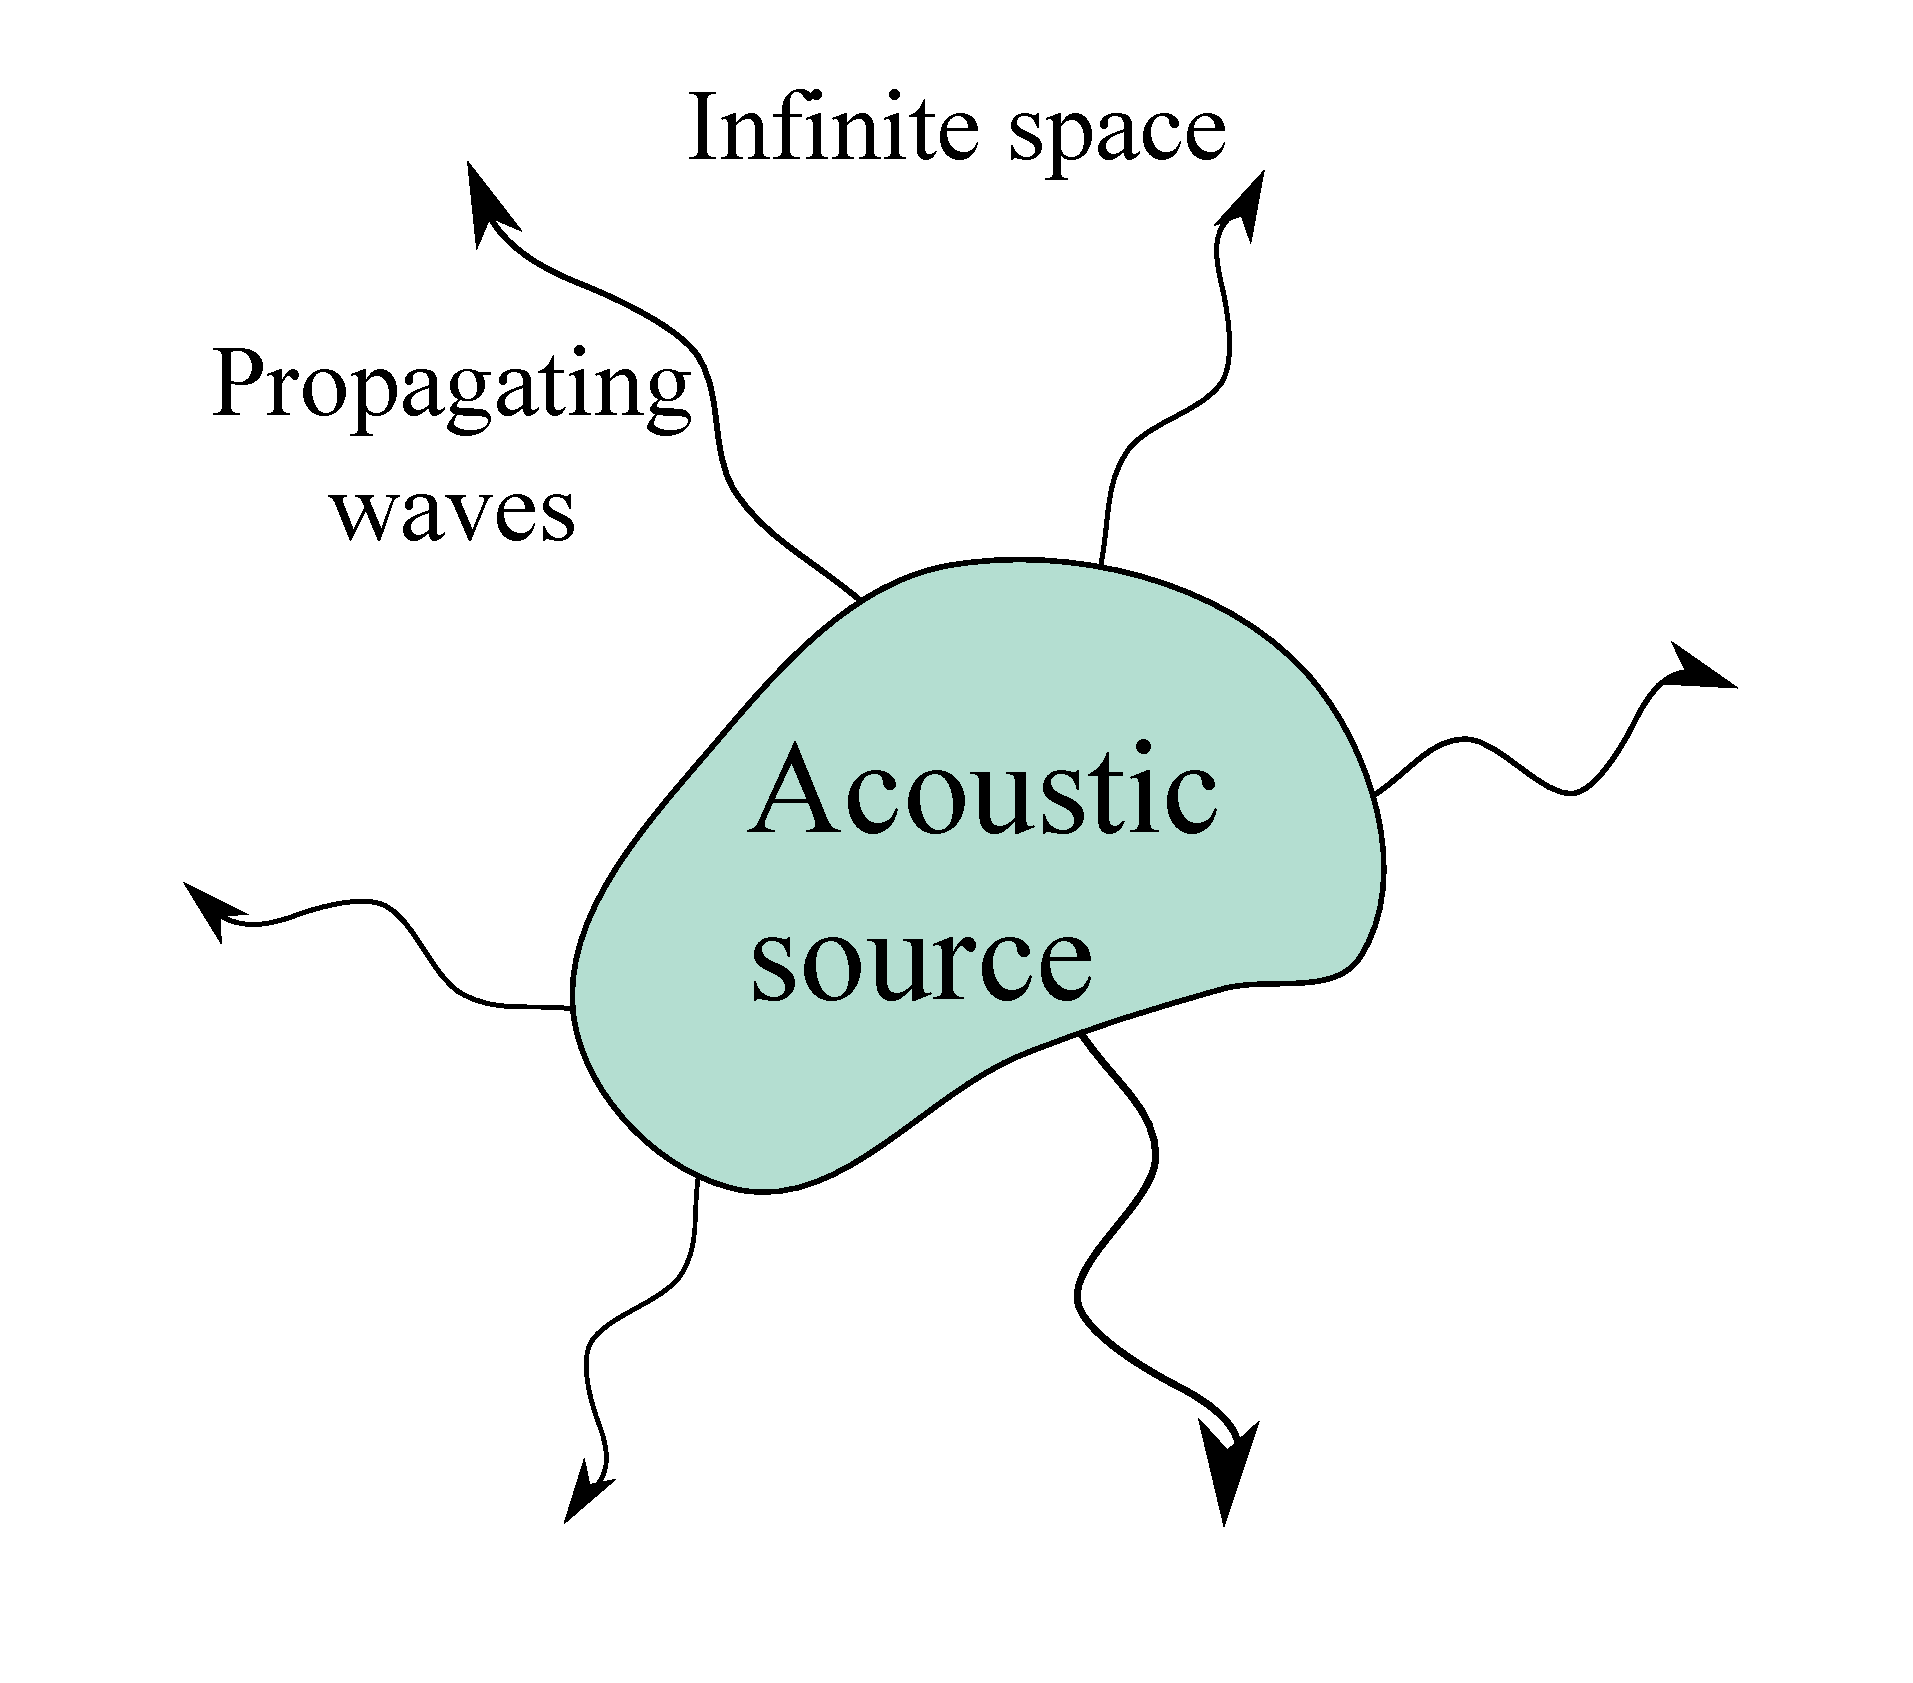
\includegraphics[width=7cm]{Figures/IntroBackground/UnboundedRegion.eps}}
        \caption{}
        \label{fig:UnboundedDomain}
    \end{subfigure}
    \hfill
    \begin{subfigure}[h]{0.47\textwidth}
        \centering
        \makebox[0pt]{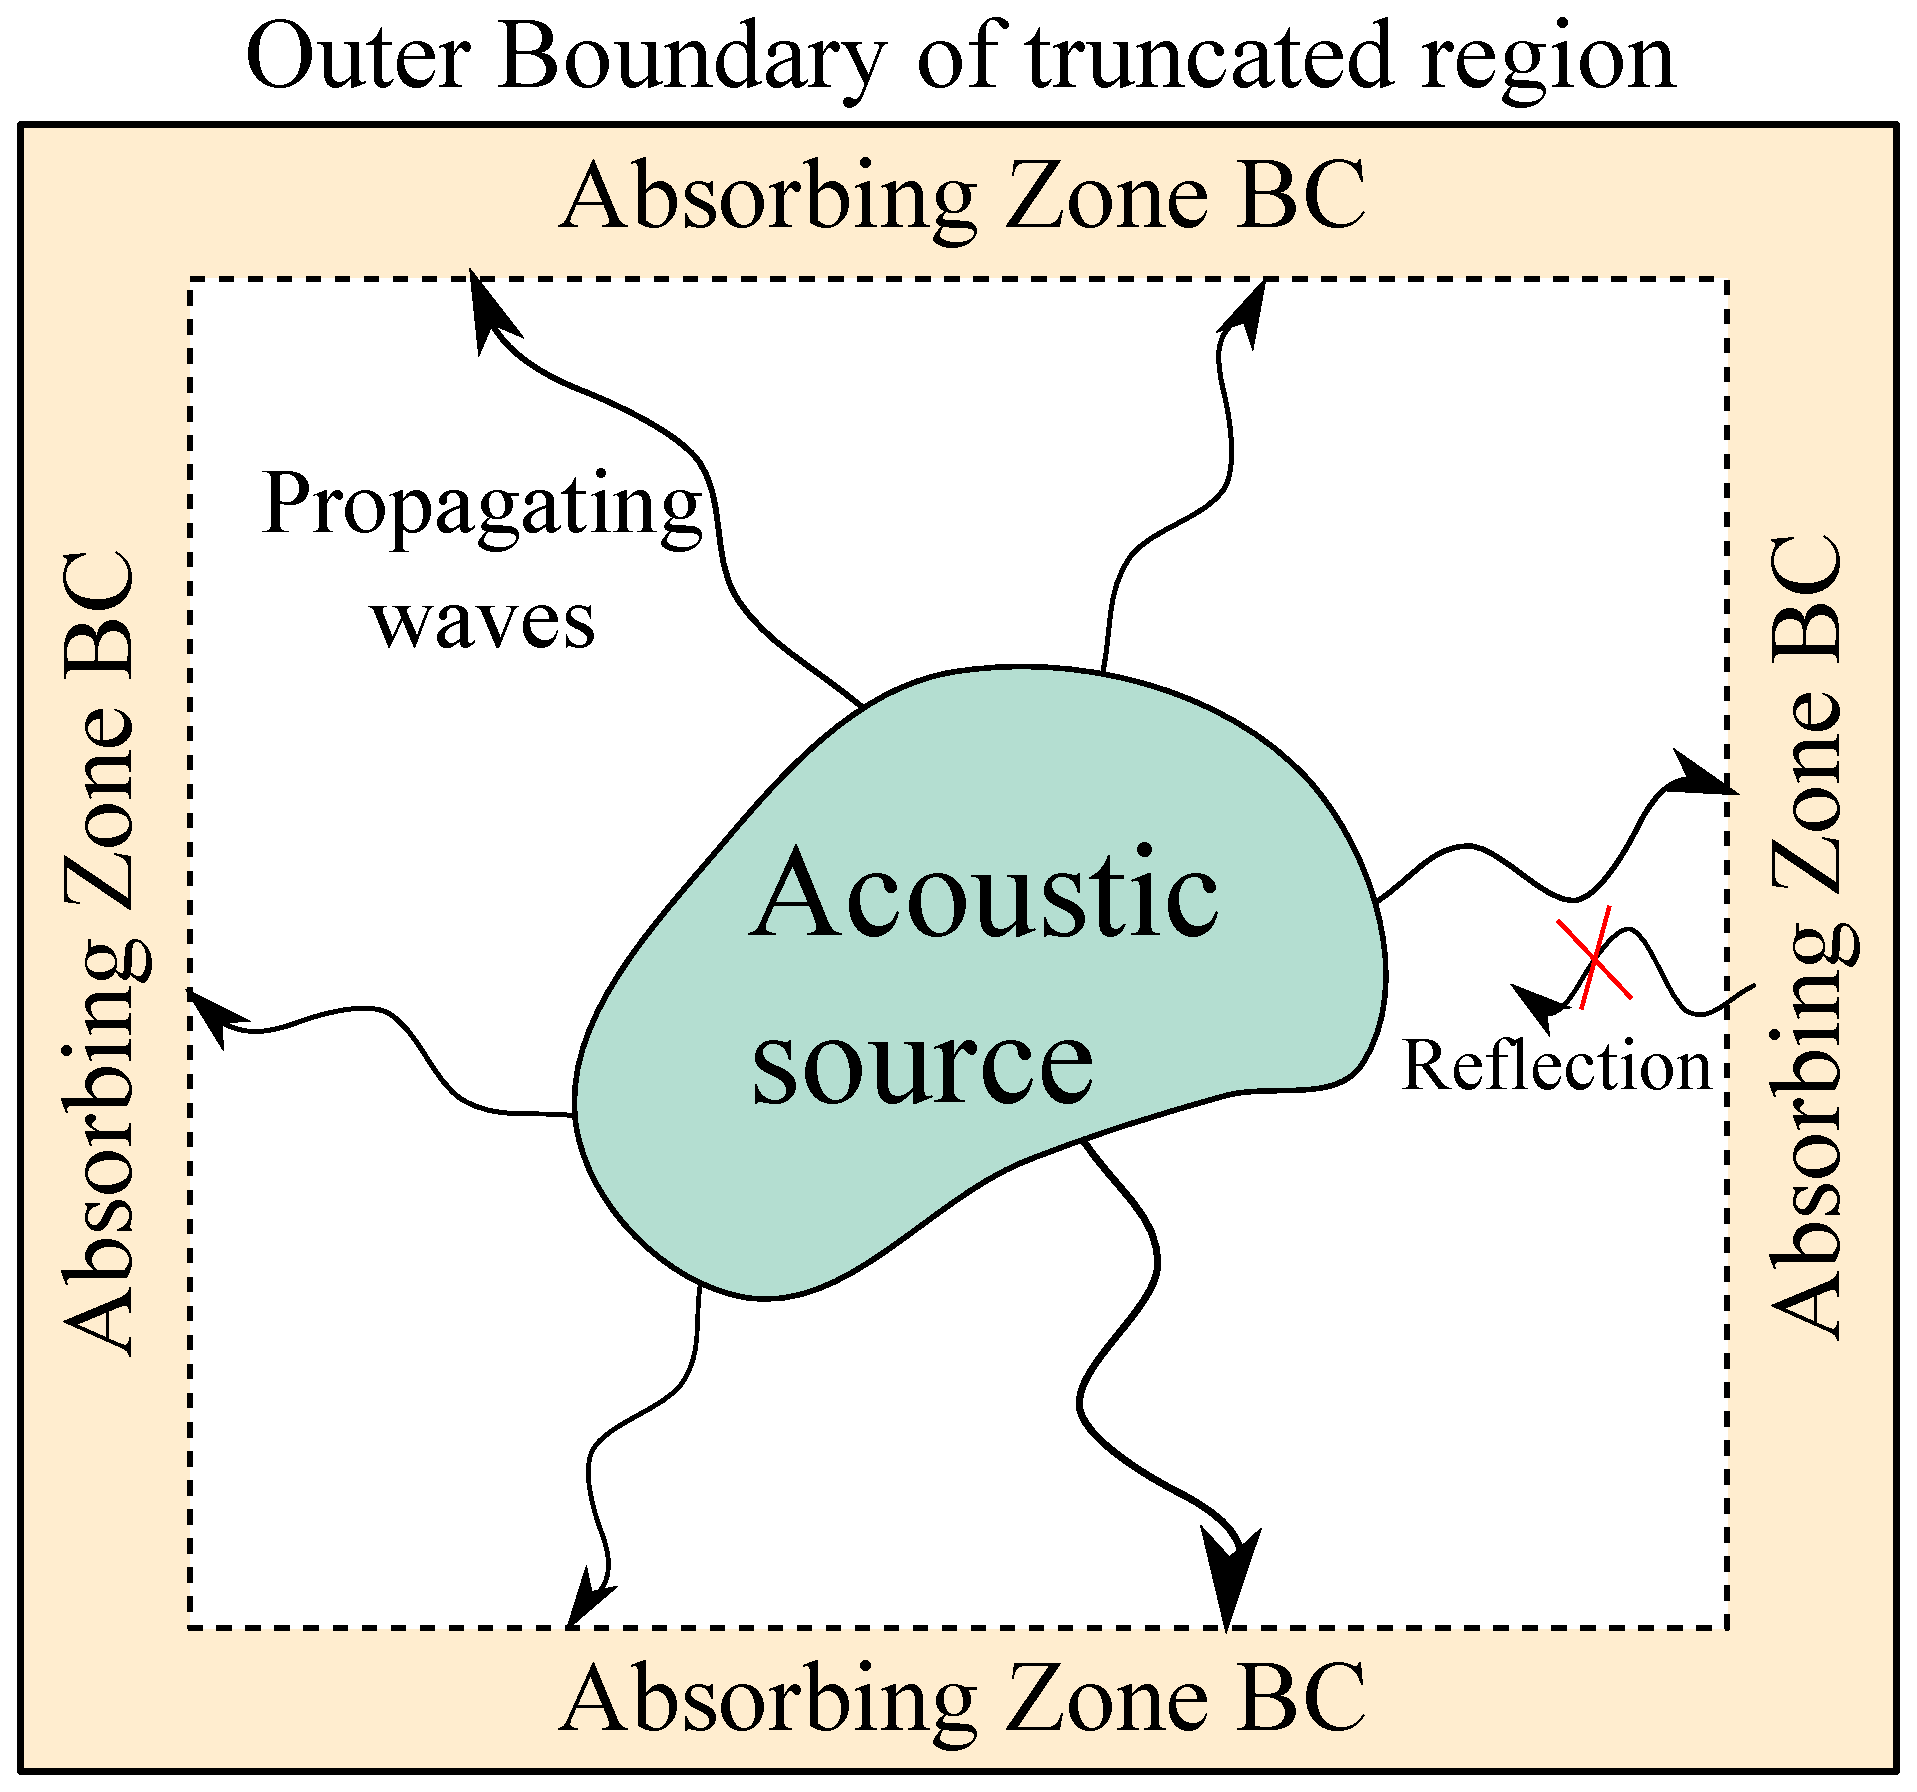
\includegraphics[width=7cm]{Figures/IntroBackground/TruncatedRegion.eps}}
        \caption{}
        \label{fig:TruncatedDomain}
    \end{subfigure}
    \caption{Simplified solution space, with a finite inner region of interest containing an acoustic source. (\textbf{a}) shows propagating waves extending to infinity, and (\textbf{b}) shows a truncated region with an absorbing zone boundary condition where propagating waves are damped to inhibit reflections \& error in the inner domain.}
    \label{fig:Domain}
\end{figure}


\textcite{kim2000generalizedcharbc} group NRBC's into 3 main types. The first are formulations based on the characteristic directions of governing equations, but these are quickly dismissed for the CAA application due to the ineffectiveness for waves impinging on the boundary at any varying angle, as described by \textcite{colonius2004modelling}. The second are formulations based on the asymptotic solution of the governing equations, where the equations are solved in the farfield for a uniform flow. \textcite{bayliss1982farfield} conclude that the asymptotic BC requires the farfield be placed sufficiently far to achieve accuracy comparable to other BCs mentioned here. This increases the computational cost and hazes the applicability with regards to what domain size is suitable. The final type of NRBC are formulations based on damping/buffer/sponge zones being added to the boundary, where the incident waves are filtered/stretched/damped to prevent reflections. This type of NRBC is by far the most applicable and does not depend on the flow characteristics - as the first type does.

There are a number of damping zone non-reflecting boundary conditions that have been formulated for methods which solve both linearised and nonlinearised Euler equations. Three have been identified from literature as potential solutions.
The PML method, originally derived as a solution for Maxwell's equations by \textcite{berenger1994apml} and adapted for aeroacoustics by \textcite{hu1996onabsorbingbc} \cite{hu2001astablePML} \cite{hu2005aPML}, is a strong version of the damping zone NRBC which absorbs out-flowing waves at domain boundaries by constructing modified governing equations (differently to the earlier NRBCs) with an additional dissipation term. The original aeroacoustic formulation was plagued by numerical instability, but was later amended in \cite{hu2005aPML} by aligning the group and phase velocities using a space-time transformation.

A second formulation of damping zone NRBC is the Buffer Zone (BZ), formulated by \textcite{wasitho1997simulationtfsei}, which is in fact very similar to the PML NRBC where the out-flowing waves in the buffer zone are damped as determined by a damping function. The exact formulation and method of numerical damping is slightly different to the PML and is an effective NRBC in its own right.


The final formulation of damping zone NRBC is the Energy Transfer and Annihilation (ETA), formulated by \textcite{edgar2012generalbufferzone}, which is based on stretching and filtering of the grid. As in, the energy content of the waves entering the NRBC is transferred to higher wavenumber waves using stretching of the grid. These are then subsequently eliminated using high-order numerical filtering which targets the higher wavenumbers.


\textcite{manco2019comparativesnrbc} make comparisons between the NRBC's for three different flow problems: linearised Euler equations in uniform flows, linearised Euler equations in non-uniform flows, and nonlinear Euler equations for mixing layer-type flows. For simplification, the project will opt with the linearised Euler equations in uniform flow case. The author concludes that the ETA NRBC is not as accurate as the PML or BZ - and supports more reflections as the wavefront propagates towards the boundary. The PML and BZ are reported to be very evenly matched when instantiated with similar parameters, and also happen to compute in similar CPU times. Given the application and prevalence of the PML in literature, it is the chosen NRBC.

On the topic of PML application, it's use is apparent throughout wave-type problems - both in research and in industry. For example, in electromagnetics it has been used for modelling marine controlled source electromagnetics to map ocean subsurface topology (\textcite{li2017marineCSEM}), and in aeroacoustics it has been used for developing an adjoint CAA solver for optimising acoustic liners (\textcite{ozkaya2016adjointcaaliner}). Typically, any mention of setting 'optimal' PML parameters is scarce, and where it has been mentioned, it is hastily handled by setting very large widths effectively dismissing potential efficiency gains.


Within current literature, there exists 4 papers which explore optimisation of PML performance \cite{choung2018nonreflective}\cite{li2003optimizationPML}\cite{margengo1999optimumpml}\cite{agrawal2004pmlperformance}. The latter 3 of which look to investigate the effects of the PML parameters via numerical means, albeit considering them exclusively - disregarding the relationship between damping coefficient and PML width. These 3 papers also originate in the late 1990's / early 2000's and are solely concerned with elastodynamics and electromagnetics, decreasing their relevance for the suggested application due to differing governing equations and domain setup. The first paper \cite{choung2018nonreflective} is the most recent (and only) piece of research to analytically optimise the PML parameters. The researchers assume that there are two factors inducing error within the domain: spurious waves from too small of a PML, causing discontinuous damping, and spurious waves from too little damping (defined by the coefficient), so that waves are not fully decayed by the end of the PML. These factors are proven to be intrinsically linked in that a change in one parameter might mean the other could be smaller/more efficient (e.g. the same damping coefficient might be suitable for a thicker PML, but produces errors for a thinner PML). 

One drawback of the analytical derivation \cite{choung2018nonreflective} is the underlying assumption that the induced error is only caused by two factors, which implies the mechanisms and interactions of the PML BC with the domain are fully understood to the letter\footnote[1]{one might be dubious to this fact}. This leads on nicely to \textit{numerically} optimising the PML parameters in this project through design sweeps, knowing there is a source of published analytical optimums to contrast and compare against. This project is mainly focused on optimising the PML performance, not necessarily comparing it to other boundary conditions in its effectiveness.

It should be noted that at the time of writing, \cite{choung2018nonreflective} is yet to be cited and so the resultant optimal conditions have not been formally used in a CAA solver implementing PML boundary conditions.


\textbf{Literature review findings:}
\begin{itemize}
    \itemsep0em
    \item Characteristic, asymptotic, and damping zone non-reflecting boundary conditions for CAA
    \item 3 damping zone non-reflecting boundary conditions (Perfectly Matched Layer, Buffer Zone, Energy Transfer and Annihilation) which outperform characteristic and asymptotic BCs
    \item 4 papers exploring optimisation of PML performance
    \item 1 out of the 4 is concerned with aeroacoustics, and considers all the parameters inclusively
    \item Only analytical methods were used in the paper to find optimal PML conditions, opening a door for numerical methods in this project
\end{itemize}

\clearpage

\section{Technical Achievement} \label{TechnicalAchievementSection}

\subsection{Governing Equations}


Within this project, only the propagation of waves into the farfield is of interest. Thus, the viscous effects of the flow can be considered 2nd order as a source of sound - and can therefore be neglected from the governing equations. This largely simplifies the CAA approach and means the Linearised Euler Equations (LEE) can be used. Had the project required significant work on modelling the noise source, full nonlinear solutions such as DNS, LES, and DES would be required for the source zone.

As described in the Background section (Section \ref{BackgroundSection}), the hybrid CAA method allows for the wave propagation to be solved by assuming the acoustic values are a small, linear, unsteady perturbation on the steady mean flow. Thus, the Euler Equations are first presented in two-dimensional, conservative form with Cartesian coordinates as

\begin{equation}
    \frac{\partial \mathbf{U}}{\partial t} + \frac{\partial \mathbf{E}_{e}}{\partial x} + \frac{\partial \mathbf{F}_{e}}{\partial y} = 0
\end{equation}
where
\begin{displaymath}
\mathbf{U} = 
\begin{bmatrix}
\rho \\
\rho u \\
\rho v \\
\rho e_{T}
\end{bmatrix}, \quad
\mathbf{E}_{e} = 
\begin{bmatrix}
\rho u \\
p + \rho u^2 \\
\rho u v \\
u \left(\rho e_{T} + p \right)
\end{bmatrix}, \quad
\mathbf{F}_{e} = 
\begin{bmatrix}
\rho v \\
\rho v u \\
p + \rho v^2 \\
v \left(\rho e_{T} + p \right)
\end{bmatrix}
\end{displaymath}
\begin{displaymath}
e_T = e + \frac{u^2 + v^2}{2}, \quad e = \frac{p}{\rho \left(\gamma - 1 \right)}
\end{displaymath}




Which can be refactored by assuming the flow variables can be written as the sum of the mean quantity and the perturbation quantity, i.e.  $\rho = \Bar{\rho} + \rho'$, $u = \Bar{u} + u'$, $v = \Bar{v} + v'$, and $p = \Bar{p} + p'$, to give

\begin{equation}
    \frac{\partial \mathbf{U}}{\partial t} + \frac{\partial \mathbf{E}}{\partial x} + \frac{\partial \mathbf{F}}{\partial y} = \mathbf{S}
\end{equation}
where
\begin{displaymath}
\mathbf{U} = 
\begin{bmatrix}
\rho' \\
\Bar{\rho} u' \\
\Bar{\rho} v' \\
p'
\end{bmatrix}, \quad
\mathbf{E} = 
\begin{bmatrix}
\rho' \Bar{u} + \Bar{\rho}u' \\
p' + \Bar{\rho} \Bar{u} u' \\
\Bar{\rho} \Bar{u} v' \\
\Bar{u}p' + \gamma \Bar{p}u'
\end{bmatrix}, \quad
\mathbf{F} = 
\begin{bmatrix}
\rho' \Bar{v} + \Bar{\rho} v' \\
\Bar{\rho}\Bar{v}u'\\
p' + \Bar{\rho} \Bar{v}u'\\
\Bar{v} p' + \gamma \Bar{p} v'
\end{bmatrix}
\end{displaymath}

The non-homogeneous term S on the RHS of the PDE represents distributed time-dependent sources within the domain.

The dependent variables of the Euler equations are then non-dimensionalised according to the freestream (uniform mean flow) conditions, with variables given in Table \ref{tab:DimensionlessVariables}.

\begin{table}[h]
    \centering
    \caption{Dimensionless variables and associated scales.}
    \begin{tabular}{ll}
        \hline \hline
        \textbf{Dimensionless variable} & \textbf{Scale} \\
        \hline
        $\Delta x$ & length \\
        $a_\infty$ (ambient sound speed) & velocity \\
        $\frac{\Delta x}{a_\infty}$ & time \\
        $\rho_\infty$ & density \\
        $\rho_\infty a_\infty^2$ & pressure \\
        \hline \hline
    \end{tabular}
    \label{tab:DimensionlessVariables}
\end{table}

The derivation is relatively long but trivial, and thus unsuitable for a technical report of this length (please refer to pp.14-19 of \textcite{velu2010development} for the derivation). The resultant LEE with uniform mean flow (in the x direction to increase likeness towards an engine setup) and grouped flux terms are


\begin{equation} \label{eq:LEE}
    \frac{\partial \mathbf{U}}{\partial t} + \frac{\partial \mathbf{E}}{\partial x} + \frac{\partial \mathbf{F}}{\partial y} = 0
\end{equation}
where
\begin{displaymath}
\mathbf{U} = 
\begin{bmatrix}
\rho' \\
u' \\
v' \\
p'
\end{bmatrix}, \quad
\mathbf{E} = 
\begin{bmatrix}
M \rho' + u' \\
M u' + p' \\
M v' \\
M p' + u'
\end{bmatrix}, \quad
\mathbf{F} = 
\begin{bmatrix}
\rho' + v' \\
u' \\
v' + p' \\
p' + v'
\end{bmatrix}
\end{displaymath}

 \label{GovEqSection}


\subsection{Perfectly Matched Layer Boundary Condition}

\input{Chapters/TechnicalAchievementChapters/PMLBCFolder/PerfectlyMatchedLayerMethod}

\input{Chapters/TechnicalAchievementChapters/PMLBCFolder/DispersionRelations}

\input{Chapters/TechnicalAchievementChapters/PMLBCFolder/OptimumConditions}

\clearpage



\subsection{Numerical Methods} \label{NumMethSect}

\input{Chapters/TechnicalAchievementChapters/NumericalMethodsFolder/SpatialDiscretisation}

\input{Chapters/TechnicalAchievementChapters/NumericalMethodsFolder/TemporalDiscretisation}

\input{Chapters/TechnicalAchievementChapters/NumericalMethodsFolder/CartesianGrid}

\input{Chapters/TechnicalAchievementChapters/NumericalMethodsFolder/AdditionalBCs}

\input{Chapters/TechnicalAchievementChapters/NumericalMethodsFolder/GeneralAlgorithm}



\subsection{Results}

\input{Chapters/TechnicalAchievementChapters/ResultsFolder/BenchmarkValidation}

\input{Chapters/TechnicalAchievementChapters/ResultsFolder/PMLParameters}

\input{Chapters/TechnicalAchievementChapters/ResultsFolder/CFDNoiseSolution}


\newpage

\section{Conclusion} \label{Conclusion}
The ability of a finite-difference-discretised solver to predict wave propagation and damping has been investigated, with clear positive results of recommended BC parameter combinations. The list of objectives from Section \ref{IntroductionSection} are revisited below in Table \ref{tab:ConclusionObjectives}.

\begin{table}[h]
    \centering
    \caption{Project Objectives.}
    \begin{tabular}{ll}
        \hline \hline
        \textbf{Objective} & \textbf{Achieved?} \\
        \hline
        Discretise PDEs using CAA-relevant schemes & Yes \\
        Write a linearised solver in MATLAB to predict wave propagation & Yes \\
        Implement absorbing zone NRBCs & Yes\\
        Benchmark the solver against workshop problems & Yes\\
        Determine 'optimal' NRBC parameters & Mostly \\
        \hline \hline
    \end{tabular}
    \label{tab:ConclusionObjectives}
\end{table}


The majority of the objectives have been completed in the fullest, with the exception of the final determination of 'optimal' NRBC parameters. Whilst results have been achieved, they require evaluation through another solver\footnote[2]{there does come a point though where the next solver must then be validated, and the same again, until no end. So these results are likely well-grounded}.

As described and justified in the results section, implementation of the perfectly matched layer BC in a linearised Euler CAA solver should be parameterised for efficiency with a PML width of $D_{x,y}=19 \Delta x$, and damping coefficient $2.7 \leq \sigma_{x,y} \leq 5.3$. Should absolute solver reliability and accuracy be more important than computational efficiency, it would be feasible to increase the PML width to $D_{x,y}=25-30 \Delta x$ with the same damping coefficients at a slight computational expense.


As for discretisation schemes, the dispersion relation preserving scheme by \textcite{tam193DRP} forms a self-contained spatial and temporal method and is readily applicable to various governing equations (including those augmented by boundary conditions) - making it an excellent choice for a computational aeroacoustics solver. 



The presented work indicates some limitations of the approach, and also of the selected boundary condition. For starters, the constructed domain is simplified to be only 2-dimensional, which is useful for simplifying the computational implementation but neglects potential 3D effects. Additionally, the governing equations are the linearised Euler equations, and assume linear wave propagation even for higher Mach numbers and frequencies (shorter wave components). In reality, the wave propagation contains nonlinear characteristics which must be captured by nonlinear Euler equations. The recommended parameters are also derived from the square damping profile $\Gamma$, and so might require tweaking for higher power profiles (this would only be considered should it provide greater efficiency, in which case it might only be a few grid points different). A single self-contained spatial \& temporal discretisation scheme has also been used where other schemes might predict slightly different propagation.

As for the perfectly matched layer BC itself, \textcite{johnson2021notesonPML} highlights an issue where waves at a glancing incidence might incur round-trip reflections in the absorbing zone. The exclusive application of the PML BC to the outer boundaries of the CAA domain (for this project trying to represent an open domain, not ducted) lessens this issue substantially. Additionally, the PML method is only reflectionless when solving for the exact wave equations (as discussed in Section \ref{NumMethSect}) - and is subject to errors where finite difference schemes make approximations. Thus it's performance is not consistent across schemes.



\subsection{Further work}

First and foremost, the work carried out here may be extended by assessing the numerically derived 'optimal' parameters on a more mature research solver. As thorough as the outlined approach may be, it is still \textit{good science} to formally assess conclusive results through another medium. Additionally, further investigations might proceed in areas such as:
\begin{itemize}
    \itemsep0em
    \item Use of different FD schemes which are less common in CAA implementations. This project's approach to PML performance is fundamentally based on numerical results, and not on the wavenumber and analytical solutions.
    \item Expansion of domain geometry to be more representative of gas turbine fan ducting (shape and additional spatial dimension) - which would introduce other variables such as angle of incidence and 3D effects. The Third CAA workshop \cite{dahl2000caaworkshop} also contains problems based on engine fans.
    \item Testing of perfectly matched layer method for waves at glancing incidences.
    \item Exploration of PML as an absorbing material - to potentially be used to model liner characteristics rather than using an extended Helmholtz resonator. Could purposeful reflection be introduced?
    \item Optimisation of PML parameters for nonlinear Euler equations or even Navier-Stokes equations. Additional elements would be required such as shock handling, high-order numerical damping, and differing Euler/PML equations (PENNE equations \cite{long2000nonconservative}).
    \item On the topic of liners - using absorption to influence thermoacoustic stability of flames within combustors (very cutting-edge).
\end{itemize}


\clearpage

\printbibliography
\clearpage

\end{document}


% - Peter Cassidy